\documentclass[11pt]{report}
%\usepackage{fancybox}
\usepackage{geometry}
\usepackage{amsmath}
\usepackage{txfonts}
\usepackage{layout}
\usepackage{setspace}
%\usepackage{mathptmx}
\geometry{a4paper, left=22mm, right=22mm, top=25mm, bottom=25mm}
\usepackage{wrapfig}
\usepackage[dvipdfm]{graphicx,hyperref}
\usepackage{mediabb}
\setstretch{1.3}
\title{\Huge\bf{Role of Noncollective Excitations in Low-Energy Heavy-Ion Fusion Reaction
and Quasi-Elastic Scattering}}
\author{\\\\\\\\\\\\\\\\\\\\\\\\\\\\{\it\Large Department of Physics, Faculty of Science, Tohoku University}\\\\
\Huge Shusaku Yusa}
\date{March, 2013}
\begin{document}


\chapter{Noncollective excitations in $^{16}$O + $^{208}$Pb reaction}
In this chapter, we discuss the role of noncollective excitation of $^{208}$Pb
in $^{16}$O + $^{208}$Pb reaction
at energies around the Coulomb barrier\cite{YHR12}.
This system has been extensively studied both
experimentally and theoretically. Using the information on the noncollective
excited states in $^{208}$Pb, 
we describe the noncollective excitations in the $^{16}$O + $^{208}$Pb
reaction and investigate their effects on the reaction observables.

\section{Current status of $^{16}$O + $^{208}$Pb reaction}
The $^{16}$O + $^{208}$Pb system has been studied both from the 
theoretical and experimental sides.
The fusion cross sections for this system have been measured at
subbarrier and above barrier energies\cite{MBD99},
as well as at deep subbarrier energies\cite{DHD07}.
The coupled-channels analysis
has also been performed.
Although a careful analysis has been performed by taking into account 
vibrational excitations in $^{16}$O and $^{208}$Pb nuclei,
the experimental fusion barrier distribution
has not been well reproduced theoretically.
In Fig. \ref{fig6.1}, we show
the barrier distributions for $^{16}$O + $^{208}$Pb system given in 
Ref. \cite{MBD99}. 
The calculated barrier distributions are compared with the
experimental data. In these calculations, phonon excitations
of $^{208}$Pb are taken into account, including also
the anharmonicity of the phonon excitations 
(see the solid lines).
In Fig. \ref{fig6.1}(b), the 
excitation energy of the $3^-$ state
and the coupling strength for the 2-phonon
states are reduced.
As one can see,
the coupled-channels calculation overestimates the height of the 
main peak in the barrier distribution.
Not only fusion experiments,
but also the experiments for quasi-elastic scattering have
been performed and the quasi-elastic barrier distribution has been
extracted\cite{T96,T97,evers,lin}.
In addition, the energy dependence of the
Q-value distribution is obtained at subbarrier energies.
The experimental data of Ref. \cite{evers}
for the Q-value distribution has already been shown in Fig. \ref{fig1.4}.
The experimental data show that the contribution from the 
inelastic scattering of higher excitation energy (Q-value) becomes more and
more important as the incident energy increases, 
while at the lowest incident energy,
the contribution from the elastic channel is dominant.
As can be seen from the spectrum of $^{208}$Pb shown in Fig. \ref{fig2.4},
these higher-lying excitations are
noncollective excitations.
Since the conventional coupled-channels calculations take into account only
the low-lying collective excitations, they do not yield the Q-value spectra at
higher excitation energies, and thus the behavior of the experimental Q-value
distribution cannot be accounted for by the
conventional calculations.
\begin{figure}[t]
  \center
    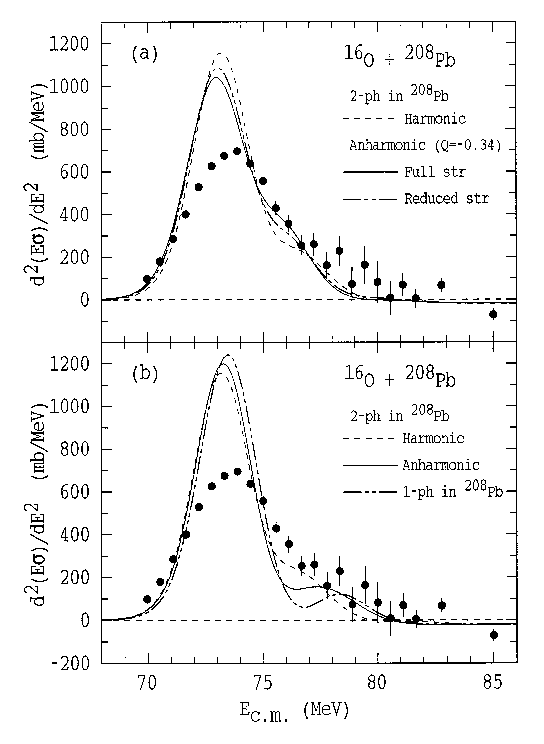
\includegraphics[clip,keepaspectratio,width=90mm]{figure/chapter6/fus_bar16O_208Pb.eps}
    \caption{Fusion barrier distribution for $^{16}$O + $^{208}$Pb system. Taken
    from Ref. \cite{MBD99}.
    The dots represent the experimental data, and lines are the results of the
    coupled-channels calculation. 
    These calculation includes phonon
    excitations of $^{208}$Pb. Anharmonicity of the phonon excitations
    is taken into account in the solid lines.
    The solid line in the figure (b)
    assumes the smaller excitation energy
    than the physical value
    and the reduced coupling strength for 2-phonon states
    from the harmonic limit.}
    \label{fig6.1}
\end{figure}

For $^{208}$Pb nucleus, the information on the excited states has been
obtained from high precision proton inelastic scattering experiments\cite{WCHM75,LBF73}
up to rather high excitation energies.
In fact, the excitation energy, spin, parity and deformation parameter are
identified with a DWBA analysis for almost all excited states up to 7.5 MeV.
We can use these information to describe the noncollective excitations in
$^{16}$O + $^{208}$Pb reaction.
By taking into account the noncollective excitations in $^{16}$O + $^{208}$Pb fusion
and quasi-elastic scattering, we investigate in this chapter 
whether the noncollective excitations
can improve the agreement of the barrier distribution with the experimental data.
We also calculate the energy dependence of the Q-value distribution and see 
whether the tendency of the experimental data can be reproduced.

\section{Results}
We now numerically solve the coupled-channels equations
for the $^{16}$O + $^{208}$Pb reaction.
For the coupling to the collective excitations, we take into account the
vibrational $3^-$ state at 2.615 MeV, $5^-$ state at 3.198 MeV, and 2$^+$ state
at 4.085 MeV in $^{208}$Pb 
(see Table 2.1) as well as the $3^-$ state at 6.13 MeV in $^{16}$O.
The deformation parameters are estimated from the measured 
electromagnetic transition probabilities, that is, 
$\beta_3 (^{208}$Pb) = 0.122, 
$\beta_5 (^{208}$Pb) = 0.058, 
$\beta_2 (^{208}$Pb) = 0.058, and
$\beta_3 (^{16}$O) = 0.733, 
together with a radius parameter 
of $r_0$=1.2~fm. 
In addition to these collective vibrational states, we also include
70 noncollective states in $^{208}$Pb below 7.382~MeV 
(see Fig. \ref{fig2.4}),  
whose excitation energies, multipolarities, and
deformation parameters are taken from the high-resolution proton
inelastic scattering measurements in Ref.~\cite{WCHM75}.
We take into account the mutual excitations of the $^{208}$Pb and the 
$^{16}$O nuclei. 

For the nuclear potential, 
we use the same geometry as that in 
Ref.~\cite{evers}, 
where the parameters were obtained by fitting the coupled-channels 
calculations 
to the experimental quasi-elastic scattering cross sections.
This potential has a surface diffuseness parameter of $a=0.671$~fm
and uses the radius parameter of $R = 8.39$ fm. 
Since our calculation takes into account the 3$^{-}$ state in
$^{16}$O, that was not included in Ref.~\cite{evers}, 
we modify the potential depth from 853~MeV to 550~MeV in order to 
compensate the adiabatic potential 
renormalization (see section 3.6.3)~\cite{THAB94}. 
For the form factors of the noncollective couplings, 
for simplicity we take the same geometry as that for the collective 
couplings. 
For the noncollective excitations,
we include only the couplings from the ground state,
and neglect 
the couplings among the noncollective excitations 
as well as the couplings
between the collective and the noncollective states.  

\subsection{Single phonon calculation}

We first show the results for the calculation that takes into account
only the single octupole phonon state in the $^{208}$Pb
together with the other collective and the noncollective states.
In this case, the number of
channels amounts to 146 in the isocentrifugal approximation. 


Figures \ref{fig:fusion}(a) and 
\ref{fig:fusion}(b) 
show the fusion cross sections 
thus obtained. They are 
plotted both on the linear scale (Fig.~\ref{fig:fusion}(a)) 
and on the logarithmic scale (Fig.~\ref{fig:fusion}(b)).
The corresponding barrier distributions, 
$D_{\rm fus} = d^2(E\sigma_{\rm fus})/dE^2$, are plotted in 
Fig.~\ref{fig:fusion}(c).
The experimental data are taken from Refs.~\cite{MBD99,DHD07}.
The dashed lines are obtained by taking into account only
the collective excitations of $^{208}$Pb and $^{16}$O, 
while the dot-dashed
lines take into account also the noncollective excitations of $^{208}$Pb. 
One immediately sees that 
the main peak in the barrier distribution is shifted in energy 
due to the noncollective excitations 
towards low energy and consequently the fusion 
cross sections are enhanced. 
This can be understood in terms of the adiabatic potential
renormalization because the excitation energies for the 
noncollective excitations
are relatively large. 
\begin{figure}[t]
\center
    \includegraphics[clip,keepaspectratio,width=165mm]{figure/chapter6/fus_16O_208Pb_1ph_L80_3.eps}
    \caption{ 
The fusion cross sections (Fig. \ref{fig:fusion}(a) and \ref{fig:fusion}(b)),  
the fusion barrier distribution, $D_{\rm fus} = d^2(E\sigma_{\rm fus})/dE^2$, 
(Fig. \ref{fig:fusion}(c)), and the logarithmic slope, 
$L(E) = d[{\rm ln}(E\sigma_{\rm fus})]/dE$, (Fig. \ref{fig:fusion}(d)), 
for the $^{16}$O + $^{208}$Pb reaction. 
The fusion cross sections are plotted both on the linear and logarithmic 
scales in Figs. \ref{fig:fusion}(a) and \ref{fig:fusion}(b), respectively. 
The dashed lines are obtained by taking into account only the 
collective excitations of $^{16}$O and $^{208}$Pb, 
while the dot-dashed lines take into account the 
noncollective excitations of $^{208}$Pb in addition to the collective
excitations. The solid lines are the same as the 
dot-dashed lines, but shifted in energy. 
The experimental data are taken from Refs.~\cite{MBD99,DHD07}.}
    \label{fig:fusion}
\end{figure}
One can also see that the noncollective excitations do not 
alter much the energy dependence of the fusion cross sections, as 
can be seen more clearly by shifting 
the dot-dashed lines in energy as shown in Fig.~\ref{fig:fusion} by the 
solid lines. 
As a consequence, the noncollective excitations 
hardly modify the behavior of 
the logarithmic slope, $L(E) = d[{\rm ln}(E\sigma_{\rm fus})]/dE$ (see 
Fig.~\ref{fig:fusion}(d)). 
That is, 
the calculations with only the collective excitations do not 
account for the observed large logarithmic slope at deep 
subbarrier energies. This 
remains the same even if the noncollective excitations are 
taken into account. 
This indicates that 
the deep sub-barrier hindrance of fusion cross sections cannot be 
explained simply with the noncollective excitations 
in each of the colliding nuclei, and
some other mechanism, such as noncollective excitations 
of the one-body system after the touching of the colliding nuclei, 
has to be considered~\cite{IHI09}. 

As mentioned in Sec.~I, 
it is known that the calculation with only collective excitations
does not reproduce well the experimental barrier distribution for 
this system~\cite{MBD99}. 
That is, the coupled-channels calculation yields 
a too high main peak in the barrier distribution. 
We find that the noncollective excitations are not helpful in this 
respect, as shown in Fig.~\ref{fig:fusion}(c). 
The noncollective excitations rather 
smear the barrier distribution 
at energies around 78~MeV~\cite{YHR10}, 
and the agreement is somewhat worsened. 
Clearly, one needs other mechanisms in order to 
reproduce the experimental barrier distribution for this system. 
In this connection, in the next subsection, we will investigate the effect of 
double octupole phonon excitations in $^{208}$Pb. 

\begin{figure}[t]
\center
    \includegraphics[clip,keepaspectratio,width=110mm]{figure/chapter6/fig2.eps}
    \caption{Quasi-elastic scattering cross sections
(Fig. \ref{fig:qel}(a))
    and the quasi-elastic barrier distribution (Fig. \ref{fig:qel}(b)) 
for the $^{16}$O +
    $^{208}$Pb system. The meaning of each line is the same as in
    Fig.~\ref{fig:fusion}. The experimental data are taken from Ref.~\cite{T96}.}
    \label{fig:qel}
\end{figure}



Figure \ref{fig:qel} shows the quasi-elastic scattering cross section 
and the
quasi-elastic barrier distribution, $D_{\rm qel}(E)= d[\sigma_{\rm
qel}/\sigma_{\rm_R}]/dE$ at 
$\theta_{\rm cm}=170^{\circ}$.
$E_{\rm eff}$ is the effective energy defined by Eq. (\ref{effective_E}),
which takes into account the centrifugal energy for the Rutherford trajectory.
The meaning of each line is the same as in Fig.~\ref{fig:fusion}.
The solid lines are shifted in energy with the same amount as in the fusion
calculation.
The experimental data are taken from Ref.~\cite{T96}.

One can observe 
that the change in the barrier distribution 
due to the noncollective excitations is 
similar to the fusion calculation. 
That is, 
the main effect of the noncollective excitations is 
the barrier renormalization 
without changing the shape of 
the distribution, although they smear the barrier 
distributions at 
relatively higher energies. 
The agreement with the experimental data around 
$E_{\rm eff}=75$~MeV is not improved by the noncollective excitations. 


\subsection{Double phonon calculation}

We next show the results for the calculations with the double
octupole phonon excitations 
in $^{208}$Pb.  
In this case, the number of channels included amounts to 148.
The double octupole phonon states in $^{208}$Pb have been experimentally
investigated in Refs.~\cite{YGMY96, VMA97, YKG98, VMC98, VPE01} and 
candidates for the double phonon have been 
identified. In the present calculation we assume, for simplicity, that
all four double octupole phonon states are degenerate with $E$=5.23~MeV, 
that is, twice the energy of the single-phonon state.


\begin{figure}[t]
  \center
    \includegraphics[clip,keepaspectratio,width=165mm]{figure/chapter6/fus_16O_208Pb_2ph_L80_3.eps}
    \caption{Same as Fig.~\ref{fig:fusion}, 
             but with the double octupole phonon excitations. }
    \label{fig:fusion2}
\end{figure}
\begin{figure}[t]
  \center
      \includegraphics[clip,keepaspectratio,width=110mm]{figure/chapter6/fig4.eps}
      \caption{Same as Fig.~\ref{fig:qel}, but with 
                the double octupole phonon excitations.}
      \label{fig:qel2}
\end{figure}

In Figs.~\ref{fig:fusion2} and \ref{fig:qel2}, we show the calculations
for the fusion reaction and quasi-elastic scattering, respectively.
One sees that the double phonon excitations leads only to a minor 
improvement both for fusion and quasi-elastic scattering. 
The effects of the noncollective excitations are 
similar to those in the single-phonon case presented in the 
previous subsection. 
That is, the barrier distribution is smeared above the barrier while
the shape of the lower peak is almost unchanged. 


\subsection{Anharmonicity of octupole phonon state in $^{208}$Pb}
We have also investigated the role of anharmonicity of the octupole 
phonon excitations of 
$^{208}$Pb~\cite{HTK97,zamrun}, together with the noncollective 
excitations. 
We assume that the physical octupole phonon state at $E = 2.615$ MeV is made
from the harmonic octupole and quadrupole phonons, that is,
\begin{eqnarray}
|3^{-}\rangle = \frac{1}{\sqrt{1+\alpha^2}}
\left(a_{30}^{\dagger} + \alpha\left[a_2^{\dagger}a_3^{\dagger}\right]^{(30)}
\right)|0\rangle.
\end{eqnarray}
Here, $\alpha$ is a constant and is determined from the quadrupole moment of
the octupole phonon state.
The quadrupole moment is calculated as
\begin{eqnarray}
Q_2(3^-) =
\sqrt{\frac{16\pi}{5}}
\langle 33 | Q_{20} | 33 \rangle
= \frac{3}{15\pi}eZ_{\rm T}R_{\rm T}^2\beta_2\alpha
\end{eqnarray}
or
\begin{eqnarray}
\alpha = \frac{\sqrt{15\pi}}{3eZ_{\rm T}R_{\rm T}^2\beta_2}Q_2(3^-).
\label{anharm_alpha}
\end{eqnarray}
The quadrupole moment $Q_2(3^-)$ has been measured 
experimentally
to be $Q_2(3^-) = -34\pm15e\ {\rm fm}^2
$\cite{JBF77,BH83}.
With $\beta_2 = 0.058$, $\alpha$ is then calculated
with Eq. (\ref{anharm_alpha}) to be $-0.37$.
\begin{figure}[t]
    \begin{minipage}[t]{78mm}
      \includegraphics[clip,keepaspectratio,width=78mm]{figure/chapter6/fus_16O_208Pb_beta3_0.122.eps}
      \caption{Fusion cross section and barrier distribution for $^{16}$O +
      $^{208}$Pb system.  The dashed lines
      are the results in the harmonic limit,
      while the solid lines take into account
      anharmonicity. The pink and the red lines include only the collective
      excitations and the purple and the blue lines include the noncollective
      excitations.}
      \label{anharm1}
    \end{minipage}
    \hspace{0.5cm}
    \begin{minipage}[t]{78mm}
       \includegraphics[clip,keepaspectratio,width=78mm]{figure/chapter6/qel_16O_208Pb_beta0.122_L100.eps}
       \caption{Same as Fig. \ref{anharm1}, but for quasi-elastic scattering.}
       \label{anharm2}
    \end{minipage}
\end{figure}

In the presence of the anharmonicity, $3^{-}$ state can couple to $2^+$ state
and $3^-$ state itself
(reorientation) even in the linear order in $\beta_{\lambda}$.
In fact, the matrix elements of $\hat{O}$ defined in (\ref{coupling_O}) is
given by
\begin{align}
\langle 2^+ | \hat{O} | 3^- \rangle
&= \frac{\alpha}{\sqrt{1+\alpha^2}}
  \frac{R_{\rm T}\beta_3}{\sqrt{4\pi}}
  \langle 2030 | 30 \rangle \\
\langle 3^- | \hat{O} | 3^- \rangle
&= \frac{2\alpha}{1+\alpha^2}
  \frac{R_{\rm T}\beta_2}{\sqrt{4\pi}}
  \langle 2030 | 30 \rangle.
\end{align}


In Figs. \ref{anharm1} and \ref{anharm2}, the results for the fusion reaction and 
the quasi-elastic scattering are shown respectively.
These calculations correspond to the double phonon calculation.
The pink and the red lines include only the collective excitations and the purple
and the blue lines take into account the noncollective excitations in addition
to the collective excitations.
The dashed lines are the results in the harmonic limit, and thus the same as
Figs. \ref{fig:fusion2}, and \ref{fig:qel2}.
The solid lines take into account the anharmonicity.
We can see that the effect of the anharmonicity
is quite subtle both in the fusion reaction and the quasi-elastic scattering cases,
regardless of the presence of the noncollective excitations.
Hence the improvement of the agreement with the data is not obtained
with the effect of anharmonicity.



\subsection{Q-value distribution}
Measurements of the Q-value distribution for backward-angle quasi-elastic 
scattering have been performed for this system~\cite{evers,lin}, in which
the experimental data indicate that the contribution
from the noncollective excitations increases as the incident 
energy increases. 
A big advantage of our method is that the Q-value distribution can be computed 
easily because we explicitly take into account the noncollective excitations 
in our coupled-channels calculations. 

Figure \ref{qdist_16O_208Pb} shows the Q-value distributions
at $\theta_{\rm cm}=170^{\circ}$ at six different incident
energies, corresponding to the double phonon calculations 
shown in Sec. 5.2.2. 
The spectra shown by the dashed lines 
correspond to the collective excitations while those by the
solid lines correspond to the noncollective excitations.
The envelope of the spectra is obtained 
by smearing with a gaussian function, 
\begin{eqnarray}
F(E^{*}) =
\sum_{n}\frac{d\sigma_n}{d\Omega}\,\frac{1}{\sqrt{2\pi}\Delta}e^{-\frac{(E^*-\epsilon_n)^2}{2\Delta^2}}, 
\label{eq5.6}
\end{eqnarray}
with $\Delta=0.2$~MeV. 

\begin{figure}[t]
    \includegraphics[clip,keepaspectratio,width=160mm]{figure/chapter6/fig5.eps}
    \caption{The Q-value spectra for the quasi-elastic scattering
    at $\theta_{\rm c.m.}$=170$^{\circ}$
    for the $^{16}$O + $^{208}$Pb system for six different incident energies. The
    dashed peaks correspond to the collective excitations while the solid peaks
    correspond to the noncollective excitations. The solid line is obtained by
    smearing the peaks with a gaussian function.}
    \label{qdist_16O_208Pb}
\end{figure}


Note that we include the noncollective states of $^{208}$Pb up to 
7.382~MeV. Thus the spectra above this energy correspond to
mutual excitations of the $^{208}$Pb and $^{16}$O nuclei.
One can see that, at the lowest incident energy shown in the figure, the 
contribution from the collective channels is dominant.
With increasing energy, the contribution from the noncollective
excitations becomes more and more important.
This behaviour is qualitatively 
consistent with the experimental Q-value
distribution for this system~\cite{evers,lin}.

Note that this energy dependence is 
also related to how the noncollective excitations 
modify the energy dependence of the 
barrier distribution.
Namely, at low energies where the contribution from the
noncollective excitations is not important, a change 
in the barrier distribution
is not observed. 
On the other hand, at higher energies where the
contribution from the noncollective excitations is important, the barrier
distribution is smeared due to the noncollective excitations.

\subsection{Mass-number dependence of the effect of noncollective 
excitations}

Finally, we investigate how the effect of noncollective excitations 
depends
on the mass number of the projectile nucleus. 
For this purpose, we solve the 
coupled-channels equations for the $^{32}$S + $^{208}$Pb and
$^{40}$Ca + $^{208}$Pb systems. For the nuclear potential, 
we use the Aky\"{u}z-Winther potential~\cite{Akyuz-Winther}. 
We include the same excited states in the $^{208}$Pb nucleus as those 
in the calculation for the $^{16}$O + $^{208}$Pb system discussed in the 
previous subsections. 

\begin{figure}[t]
  \begin{center}
    \begin{minipage}[t]{78mm}
      \includegraphics[clip,keepaspectratio,width=78mm]{figure/chapter6/fig6.eps}
      \caption{ Fusion cross section and fusion barrier 
                distribution for the $^{32}$S + $^{208}$Pb system.
                The meaning of each line is the same as in Fig.~\ref{fig:fusion}.
                The experimental data are taken from Ref.  ~\cite{T96}.}
    \label{fig:fusion3}
    \end{minipage}
    \hspace{0.5cm}
    \begin{minipage}[t]{78mm}
      \includegraphics[clip,keepaspectratio,width=78mm]{figure/chapter6/fig7.eps}
      \caption{ Fusion cross section and fusion barrier distribution
      for the $^{40}$Ca + $^{208}$Pb system. The meaning of each line is the same as
      in Fig.~\ref{fig:fusion}.}
    \label{fig:fusion4}
    \end{minipage}
  \end{center}
\end{figure}


We first discuss the $^{32}$S + $^{208}$Pb reaction. 
For the excitations of $^{32}$S, we take into account the 
quadrupole vibration up
to the double phonon states. The excitation energy and the 
deformation parameter are taken from Ref.~\cite{RNT01}.
Figure \ref{fig:fusion3} shows the calculated fusion cross section and fusion
barrier distribution.
The meaning of each line is the same as in Fig. \ref{fig:fusion}. 
The experimental data are taken from Ref.~\cite{T96}.
One can see that the effect of the noncollective excitations
is qualitatively similar to that in the $^{16}$O + $^{208}$Pb reaction. That is, the
barrier is shifted towards lower energy and the higher part of the barrier
distribution is smeared. However, the smearing is stronger
than that in the $^{16}$O + $^{208}$Pb system, because 
an effective coupling strength 
is in general approximately proportional to the 
charge product of the colliding nuclei~\cite{fusionbar}, and thus 
the noncollective excitations are effectively stronger
for heavier systems. 
One can also see that the two low-energy 
peaks in the barrier distribution are sharpened due to the noncollective 
excitations, while the separation between the peaks is not altered much. 
The calculations do not reproduce the experimental data, 
and this might be attributed to the role of transfer reactions. 

Figure \ref{fig:fusion4} shows the fusion cross section and the fusion barrier 
distribution for the $^{40}$Ca + $^{208}$Pb reaction. 
For this system, we assume that $^{40}$Ca is inert and take into account
only the excitations of $^{208}$Pb.
As the charge product is larger, 
the effect of the noncollective
excitations is stronger than that in the $^{16}$O + $^{208}$Pb and
$^{32}$S + $^{208}$Pb reactions. It smears the higher part of the barrier
distribution while the lower main peak is sharpened.

As we have shown, while the effect of noncollective excitations is not 
large for the $^{16}$O+$^{208}$Pb system, the effect becomes increasingly 
important for heavier systems, such as $^{40}$Ca+$^{208}$Pb. 
This suggests that the conventional coupled-channels approach, that 
neglects the noncollective excitations, is well justified for 
relatively light systems, but the noncollective excitations have to 
be included explicitly in coupled-channels calculations 
for heavy-systems, for example, those relavant to a synthesis of superheavy 
elements. 



\include{end}


